\documentclass[tikz,border=1pt]{standalone} 
\usepackage{tikz}
% \usepackage{automata, arrows}
\usetikzlibrary{arrows.meta,calc,decorations.markings,math,arrows.meta}
\usetikzlibrary{positioning}
\begin{document}
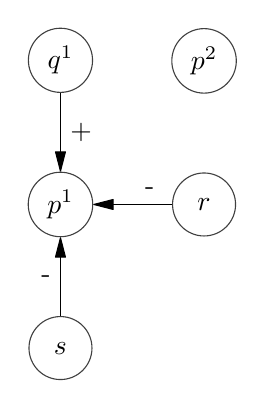
\begin{tikzpicture} [
    atom/.style={circle,  draw=black!75, minimum size=8mm},
    rule/.style={rectangle, draw=black!75, minimum size=3mm},
    sink/.style={circle, double, draw=black!75, minimum size=3mm},
    dummy/.style={midway,sloped,left,rotate=270},
    dummy2/.style={midway,sloped,left},
    >={Stealth[inset=0pt,length=8pt,angle'=28,round]}
    ]
    %Nodes
    \node[atom]      (q)                              {$q^{1}$};
    \node[atom]      (p1)       [below=of q] {$p^{1}$};
    \node[atom]      (r)       [right=of p1] {$r$};
    \node[atom]      (s)       [below=of p1] {$s$};
    \node[atom]      (p2)       [above=of r] {$p^{2}$};
    %Lines
    \draw[->] (q.south) -- (p1.north) node[dummy] {+};
    \draw[->] (s.north) -- (p1.south) node[dummy] {-};
    \draw[->] (r.west) -- (p1.east) node[dummy2, yshift=0.2cm, xshift=0.4cm] {-};
\end{tikzpicture} 
\end{document}